\section{Resultados}\label{sec:termpot}

O \emph{Termpot} (ver figura \ref{fig:termpot}) \footnote{Disponível em \url{https://jahpd.github.io/termpot}.} é uma customização do \emph{Wavepot}. Funções sonoras podem ser definidas em linguagem \emph{coffeescript} \cite{burnham2011coffeescript}, executadas e gravadas (Código 1). %\ref{code:resultados}.

\begin{figure}[!h]
\centering
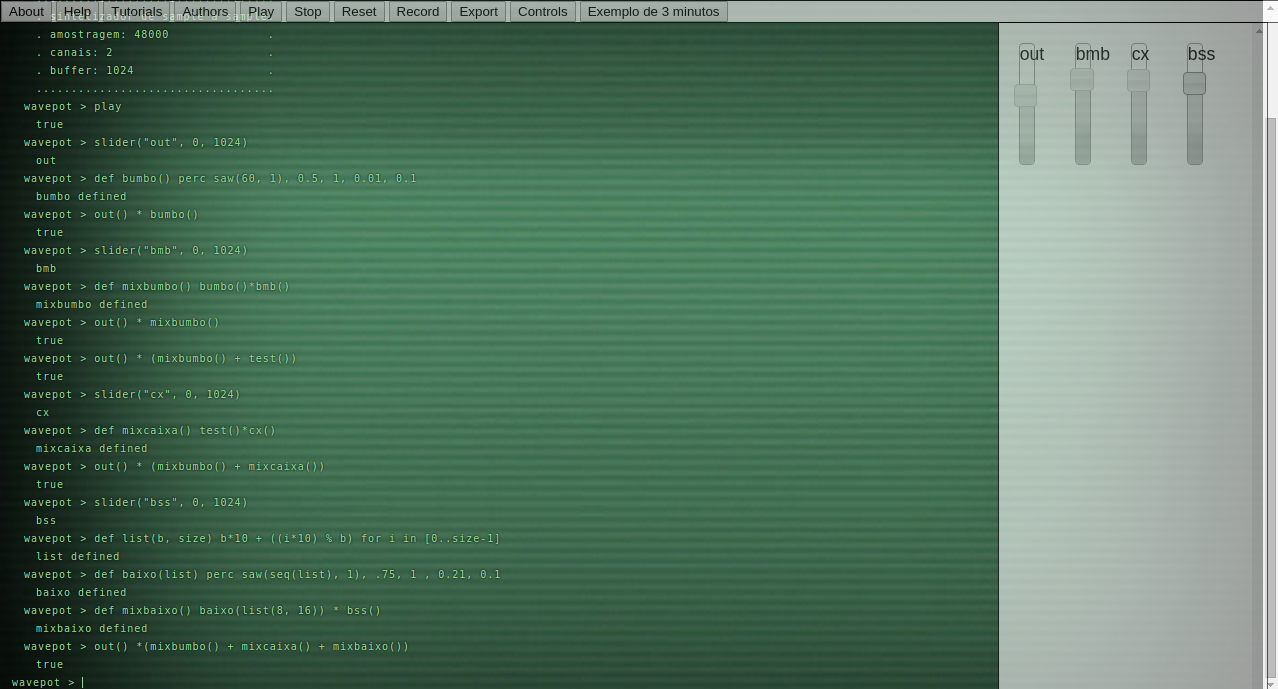
\includegraphics[scale=0.3]{termpot.png}
\caption{Aplicativo \emph{Termpot}. \textbf{Fonte}: autores.}
\label{fig:termpot}
\end{figure}

\begin{listing}
\begin{minted}[linenos,frame=lines,framesep=2mm,fontsize=\tiny]{javascript}
$ |                                                       (1)
$ wavepot 1024                                            (2)
..................................
. sintetizador de sample a sample.                        (3) 
. amostragem: 44100              .
. canais: 2                      .
. buffer: 1024                   .
..................................
wavepot > play                                            (4)                                                      
true
wavepot > def AM440(f, a) sin f1, sin(440, a)             (5)
AM defined
wavepot > inspect                                         (6)
funcoes definidas 
tau  tmod  mute  stereo  sin  sin2  saw  ramp  ttri
tri  sqr   pulse noise	 perc test  seq  bpm   nextevent
AM440
wavepot > slider "f", 1, 1025                             (7)
true
wavepot > slider "a", 0, 1024            
true
wavepot > record                                          (8)
true
wavepot > AM440 f()*1000, a()                             (9)
true
wavepot > export                                          (10)
\end{minted}
\tiny{\caption{Ptty aguardando dados de entrada do improvisador (1). \emph{Boot} do ambiente \emph{wavepot} com um buffer de 1024 amostras por ciclo de DSP (2). Informações diversas do sistema (3). Execução do DSP (4). Definição de uma função \emph{AM440} (5). Informações sobre as funções diponíveis (6). Definição de GUIs (7). Gravação em um arquivo de áudio (8). Execução da função \emph{AM440} com controles (9). Download da gravação (10)}}
\label{code:resultados}
\end{listing}

\subsection*{Problemas Técnicos}

Existem \emph{xruns}. Um \emph{xrun} ``(\ldots) pode ser um estouro de buffer ou de uma saturação de um buffer. Um aplicativo de áudio ou não foi rápido o suficiente para transmitir dados (\ldots) ou não rápido o suficiente para processar os dados" \cite{markc_xruns_2013}\footnote{Tradução nossa de \emph{An "xrun" can be either a buffer underrun or a buffer overrun. In both cases an audio app was either not fast enough to deliver data (\ldots)  or not fast enough to process data}.}. Existe uma hipótese, não verificada, que a possível fonte dos \emph{xruns} é a biblioteca \emph{jQuery}. 